\documentclass[conference]{IEEEtran}

\usepackage{graphicx}
\usepackage{xspace}
\usepackage{listings}
\usepackage[usenames, dvipsnames]{color}

\lstset{language=Python}

\lstdefinestyle{custompython}{
	belowcaptionskip=1\baselineskip,
	frame=lr,
	xleftmargin=\parindent,
	language=Python,
	basicstyle=\footnotesize\ttfamily,
	keywordstyle=\bfseries\color{MidnightBlue},
	stringstyle=\color{PineGreen}
}
         

\graphicspath{{./img/}}

\hyphenation{op-tical net-works semi-conduc-tor}


\lstset{language=Python}

\definecolor{LightGray}{RGB}{250,250,250}

\lstdefinestyle{custompython}{
	captionpos=b,                    % sets the caption-position to bottom
	% frame=tb,
	xleftmargin=\parindent,
	language=Python,
	basicstyle=\footnotesize\ttfamily,
	keywordstyle=\bfseries\color{MidnightBlue},
	stringstyle=\color{PineGreen},
  	commentstyle=\color{Magenta},
  	backgroundcolor=\color{LightGray}
}


\newcommand{\tool}{Flask Dashboard\xspace}
\newcommand{\zee}{Zeeguu\xspace}
\newcommand{\git}{\texttt{git}\xspace}
\newcommand{\install}{{\small \texttt{pip install flask\_dashboard}}\xspace}
\newcommand{\activeUserCount}{two hundred\xspace}
\newcommand{\code}[1]{\texttt{#1}\xspace}
\newcommand{\perspective}[1]{{\small {\texttt{#1}}\xspace}}

\usepackage{fourier-orns}

\definecolor{myred}{RGB}{230, 20, 70}
\definecolor{mygreen}{RGB}{60, 180, 75}


\newcommand{\niceseparator}
	{
		\begin{center}
  		% $\ast$~$\ast$~$\ast$
  		% $\clubsuit$~$\clubsuit$~$\clubsuit$
  		\leafleft
		\end{center}
	}

% Endpoint Names 
%\newcommand{\epDecoration}[1]{{\small {\bf #1}}\xspace}
\newcommand{\epDecoration}[1]{\code{#1}}

\newcommand{\epTranslations}{{\color{myred} \epDecoration{api.get\_possible\_translations}}\xspace}
\newcommand{\epOutcome}{\epDecoration{api.report\_exercise\_outcome}}
\newcommand{\epFeedItems}{\epDecoration{api.get\_article\_difficulties}}



% Author Comments / Discussion

\definecolor{mlcolor}{RGB}{140, 140, 205}
\definecolor{vacolor}{RGB}{255, 0, 255}

\newcommand{\ml}[1]{ 
	{\footnotesize \color{mlcolor}ML: #1}
	}

\newcommand{\va}[1]{ 
	{\footnotesize \color{vacolor}VA: #1}
}


\newcommand{\mltp}[1]{\ml{Thijs, Patrick: #1}}
\newcommand{\mlv}[1]{\ml{Vasilios: #1}}

\definecolor{todocolor}{RGB}{200, 140, 160}

\newcommand{\todo}[1]{ 
	{\footnotesize \color{todocolor}Todo: #1}
	}

\newcommand{\Fref}[1]{Fig.~\ref{#1}}
\newcommand{\Sref}[1]{Sec.~\ref{#1}}




\begin{document}
%
\title{Visualizing Evolving Service Performance in Python }
% Alternative Titles: The Importance of Visualization in the Performance Monitoring of Python Web Services


% author names and affiliations
% use a multiple column layout for up to three different
% affiliations
\author{\IEEEauthorblockN{Michael Shell}
\IEEEauthorblockA{School of Electrical and\\Computer Engineering\\
Georgia Institute of Technology\\
Atlanta, Georgia 30332--0250\\
Email: http://www.michaelshell.org/contact.html}
\and
\IEEEauthorblockN{Homer Simpson}
\IEEEauthorblockA{Twentieth Century Fox\\
Springfield, USA\\
Email: homer@thesimpsons.com}
\and
\IEEEauthorblockN{James Kirk\\ and Montgomery Scott}
\IEEEauthorblockA{Starfleet Academy\\
San Francisco, California 96678--2391\\
Telephone: (800) 555--1212\\
Fax: (888) 555--1212}}



% make the title area
\maketitle

\begin{abstract}
The abstract goes here.
\end{abstract}

% no keywords

\IEEEpeerreviewmaketitle



\section{Introduction}
Every system is a distributed system nowadays \cite{}. 

% \hfill mds
 
% \hfill August 26, 2015

Python is currently one of the most popular programming languages for API web service development. It was the \todo{nth} most popular programming language in the year \todo{2017/16?}

Flask is one of the two most popular web frameworks for Python. It is a lightweight alternative to web site and service development. This is why it is advertised as a {\em micro-framework}. The popularity of Flask is hinted at also by the large number \mltp{can we find an estimate on GH?} of open source projects that are hosted on GitHub which are based on it. 


However, there is no dedicated solution for monitoring the performance of Flask web-applications. Thus, every one of those \todo{NNNN} has one of the following options when confronted with the need of gathering insight into the runtime behavior of their service: 

  \begin{enumerate}

    \item use a heaviweight professional API monitoring setup they require setting up a different server \mltp{can we find a few examples of professional but overkill tools? ideally they require setting up a bunch of servers, and writing configs in XML!}. 

    \item implement their own analytics tool 

    \item do not visualize their service and lack the insight into the performance of their services.

  \end{enumerate}

For projects which are done on a budget (e.g. research projects) the first and the second options are often not available due to time and financial constraints. 

To avoid these projects ending up in the third situation, in this paper we present a low-effort, lightweight service monitoring API for Flask and Python web-services.


Architecture: series of web and mobile applications built aroud a core web service implemented in Python and Flask which provides: 
\begin{itemize}
  \item contextual translations 
  \item reading recommendations
  \item exercises
\end{itemize}



We have this system for helping learners read texts that they like, and enable them to practice with exericses generated on their past readings.



Our Solution: three lines of code that one must add to their Flask-enabled code:

\mlv{do you know how to style the code env to make it look nicer? }
\ml{see below/above}
\mltp{fix this example pls}
\begin{lstlisting}[float,caption=TBA,style=custompython]
import dashboard

dashboard.config.from_file('d.cfg')
dashboard....

\end{lstlisting}

And a small configuration file: 

\mltp{example of minimal (the most minimal possible, we'll introduce later extra configs) config file.}

\mltp{a small description of how the dashboard automatically intercepts the calls to the various API calls}

\mltp{metion also that the dashboard automatically is available at /dashboard endpoint}

\mltp{a small screenshot of how the dashboard allows one to select the interesting }

\section{Case Study}

Zeeguu case study description to be used as running example throughout the rest of the paper

\ml{we should consider adding also one section in which the architecture/implementation and main features of the dashboard are presented before going on with discussing them in more depth in the following sections}

\section{Overall Endpoint Utilization}

  The most basic insights that a service maintainer must answer regard the utilization of their service. \tool presents two perspectives that provide insight into this question. 


  Figure \ref{fig:aeu} shows the usage of the services on a daily basis while highlighting the contribution of the individual endpoints\footnote{We recommend obtaining a color version of this paper for better readability}. 

  One can see that the service at its peak has about 2500 hits per day. Moreover, one can see the way the users are using the platform since the different endpoints are indicators of different activity types, e.g.: 

  \begin{itemize}

    \item {\color{myblue}\epTranslations} is an indicator of the amount of reading the users are doing

    \item {\color{myviolet} \epOutcome} is an indicator of the amount of vocabulary practice the users are doing

  \end{itemize}




  \begin{figure}[h!]
    \centering
    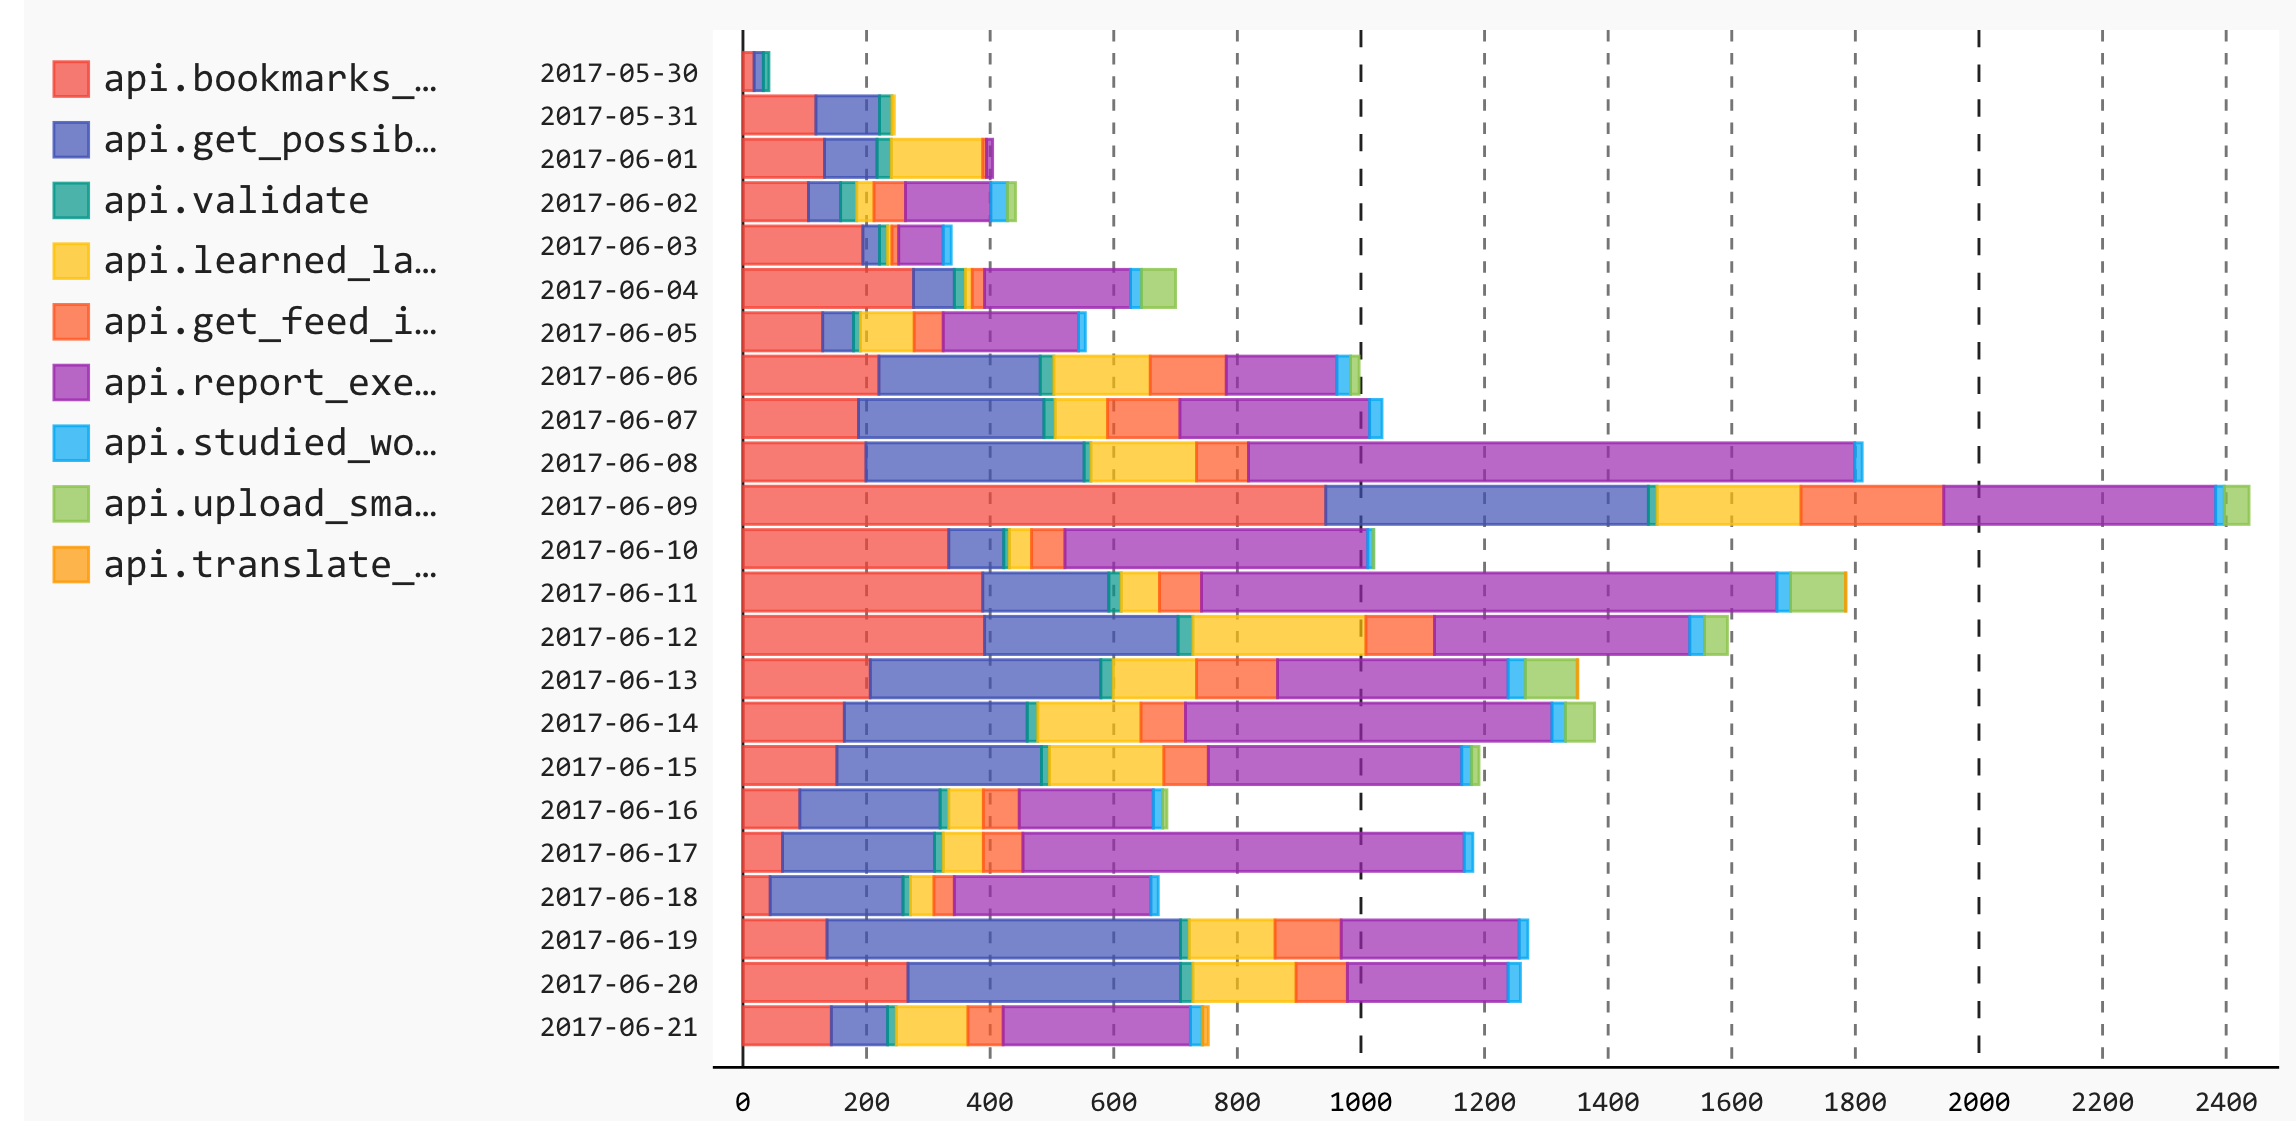
\includegraphics[width=\linewidth]{all_endpoints_usage.png}
    \caption{Caption here}
    \label{fig:aeu}
  \end{figure}

  Besides showing which endpoints are used, this view is informative for the maintainer since it provides insight into which endpoints are used. In our case study, the maintainer of the API has decided to not remove several endpoints when they saw that that were being used \footnote{Usage information can also be used to increase the confidence of the maintianer that a given endpoint is not used}

  \niceseparator

  A second question that an API maintainer must answer regards cyclic patterns of usage. 

  \mlv{can we provide some support for this claim? a reference maybe?}

  \mltp{ can we add vertical lines that highlight the beginng of a new week (e.g. before Sunday): 

  }

    \begin{figure}[h!]
      \centering
      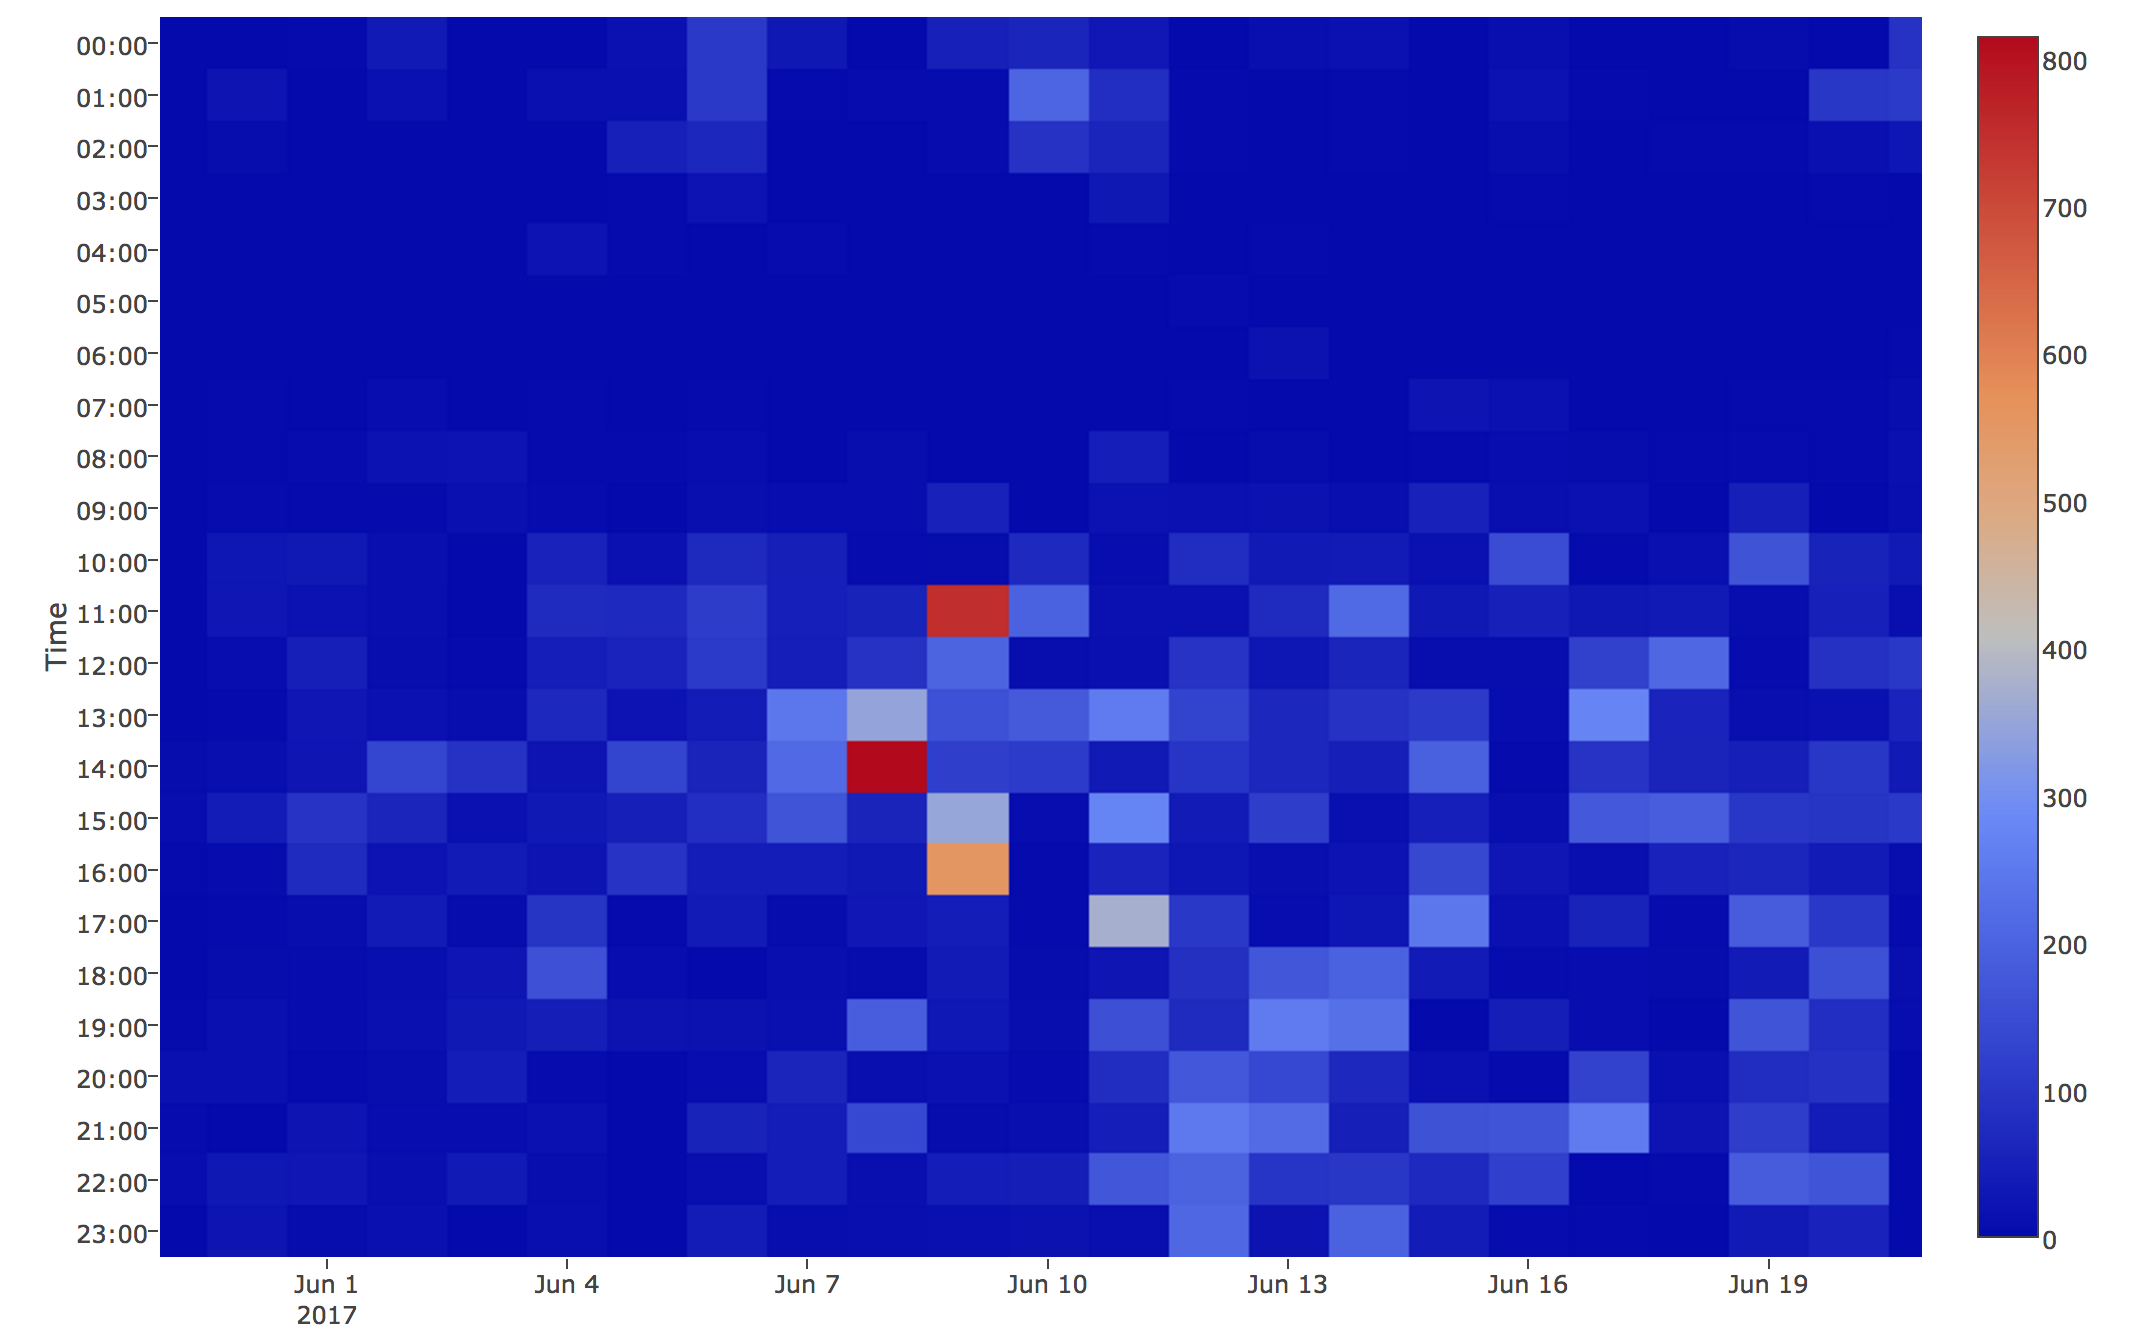
\includegraphics[width=\linewidth]{daily_patterns}
      \caption{Caption here}
      \label{fig:dp}
    \end{figure}


  Figure \ref{fig:dp} shows only one clear pattern: the users of our API do not practice foreign languages as night. Besides that, the API is used around the clock with usually a few hundred hits per hour. So the load currently is not that high. 



\section{Visualizing Service Performance}

  Another type of information that \tool can collect regards endpoint performance. Figure \ref{fig:ep} shows a summary of the response times for various endpoints by using boxplot graphs. 

  % \ml{Thijs and Patrick... the visualization people will complain when they see that we have different colors for the same endpoint in different graphs. Can we insure that there is consistency in colors? Simplest trick would be to obtain the color by hashing the name of the endpoint... in that case the same endpoint woudl have the same color in various graphs.}

  \begin{figure}[h!]
    \centering
    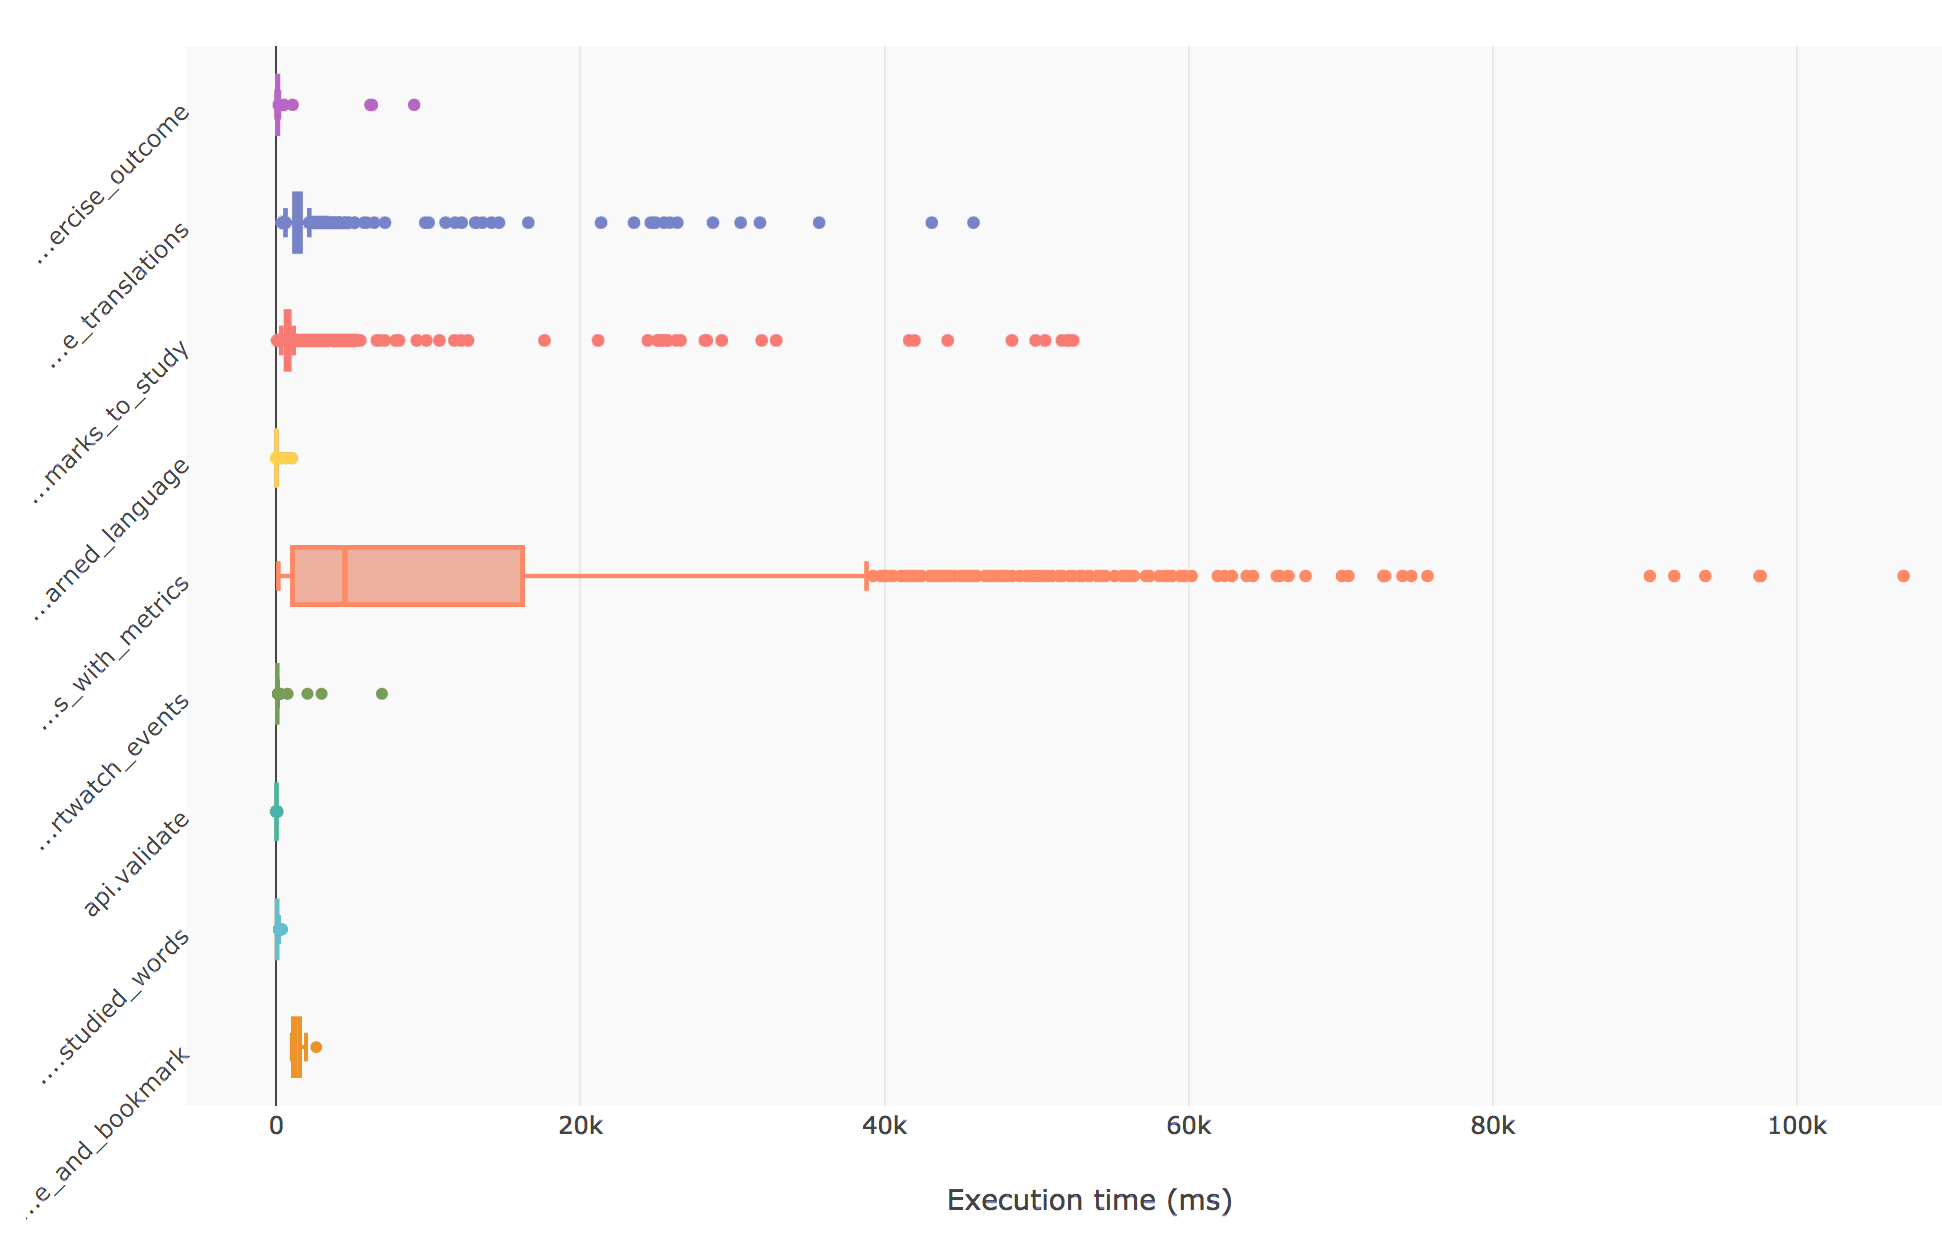
\includegraphics[width=\linewidth]{endpoint_performance.png}
    \caption{...}
    \label{fig:ep}
  \end{figure}

  After investigating this view it became clear to the maintainer that three of the endpoints had very large variation in performance. One of the most important endpoints that they decided to improve the performance of is the second from the top in Figure \ref{fig:ep}: the endpoint that returns translations. This is particularily critical since it is part of a live interaction loop. 

  \niceseparator

  Once they increased the performance of the endpoint, the maintainer realized that this graph was not that useful anymore. Because they could not see the improvements. 

  For such situations, \tool provides an extra configuration directive:

 \mltp{Add extra config line here}

  If the directive is enabled, the performance data is grouped by commit and commits are detected by analyzing the .git folder on the machine. 

  Figure \ref{fig:tee} shows the performance of the give endpoint 

  \begin{figure}[h!]
    \centering
    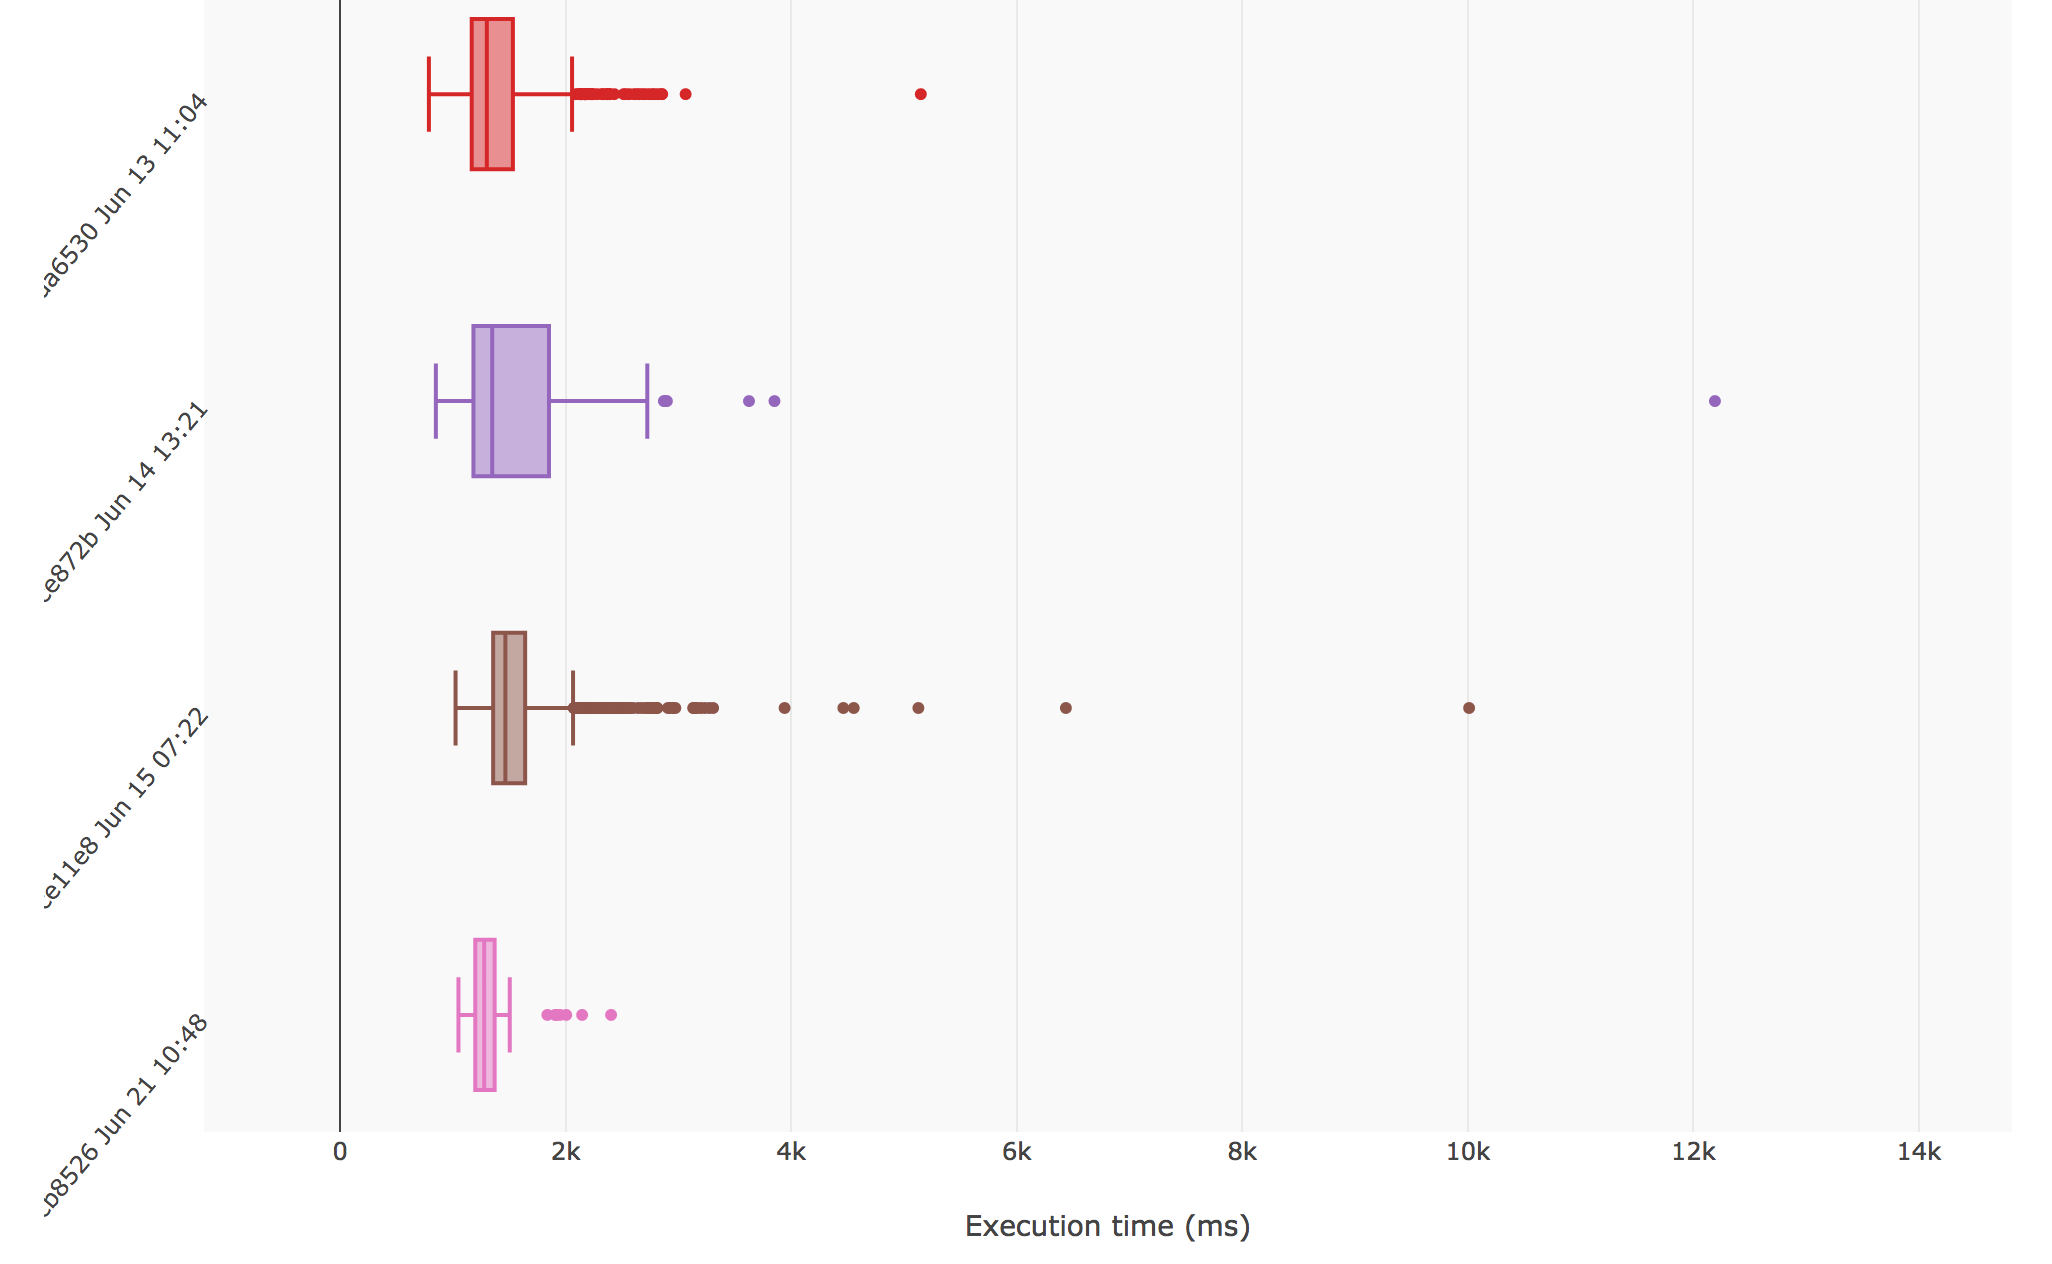
\includegraphics[width=\linewidth]{translation_endpoint_evolution.png}
    \caption{Visualizing The Performance Evolution of the \epTranslations endpoint (the second from the top in Fig. \ref{fig:ep})}
    \label{fig:tee}
  \end{figure}

  This is important since only this way can confirm that our performance improves. 



\newpage
\section {User Centered Visualization}

  Different users might have different experiences: 
  - a user has 10K emails one has 10 emails
  - a user is subscribed to 20 feeds one to 2 feeds

  The system will have different processing times. 
  It is important for the DevOps-er to be able to understand the difference in performance on a per user basis. 

  \begin{figure}[h!]
    \centering
    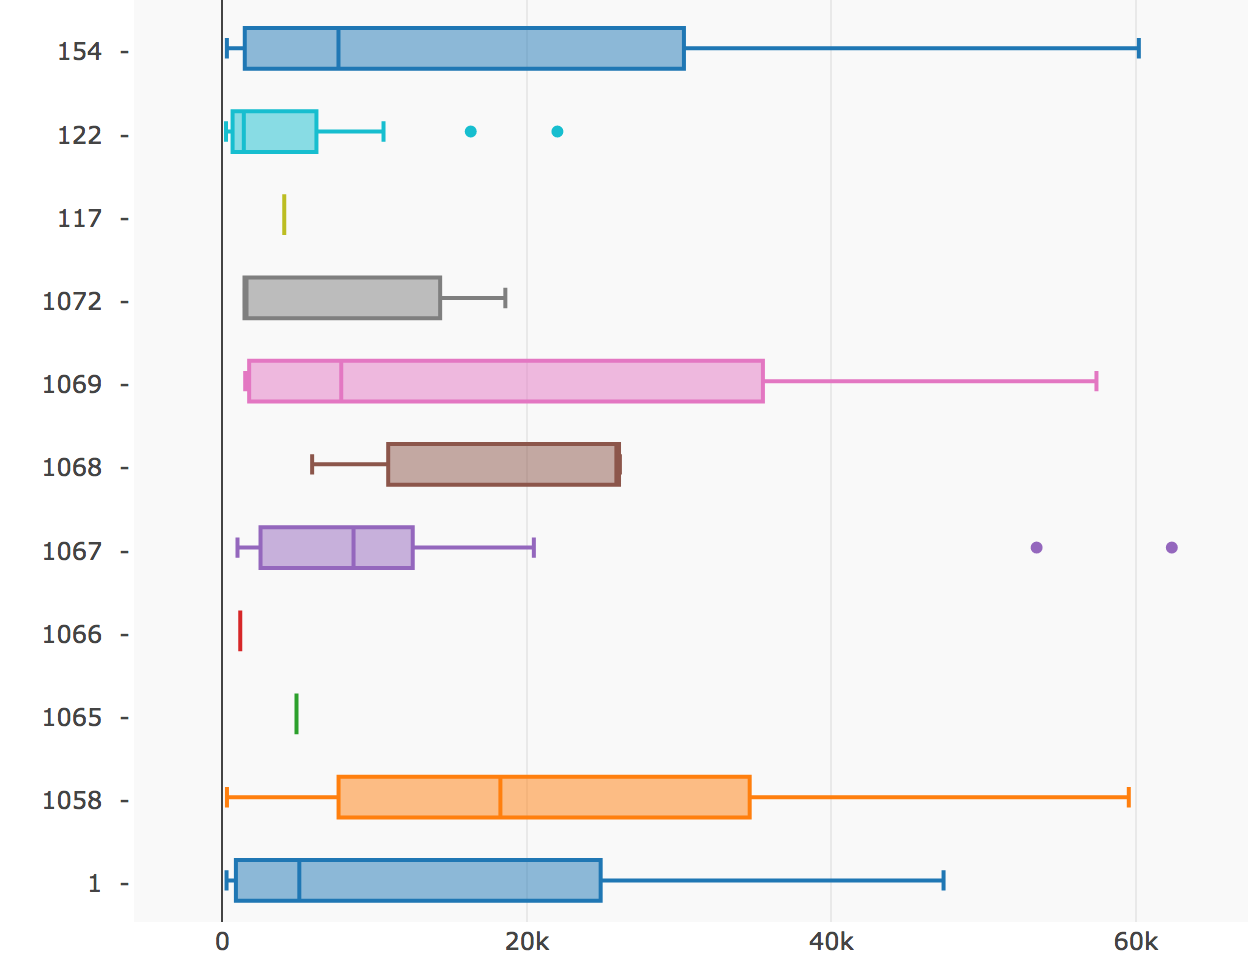
\includegraphics[width=\linewidth]{time_per_user}
    \caption{One of the endpoints (/get\_feed\_items\_with\_metrics) shows a very high variability across users}
    \label{fig:tpu}
  \end{figure}

  If we try to show also per version: 

  \begin{figure}[h!]
    \centering
    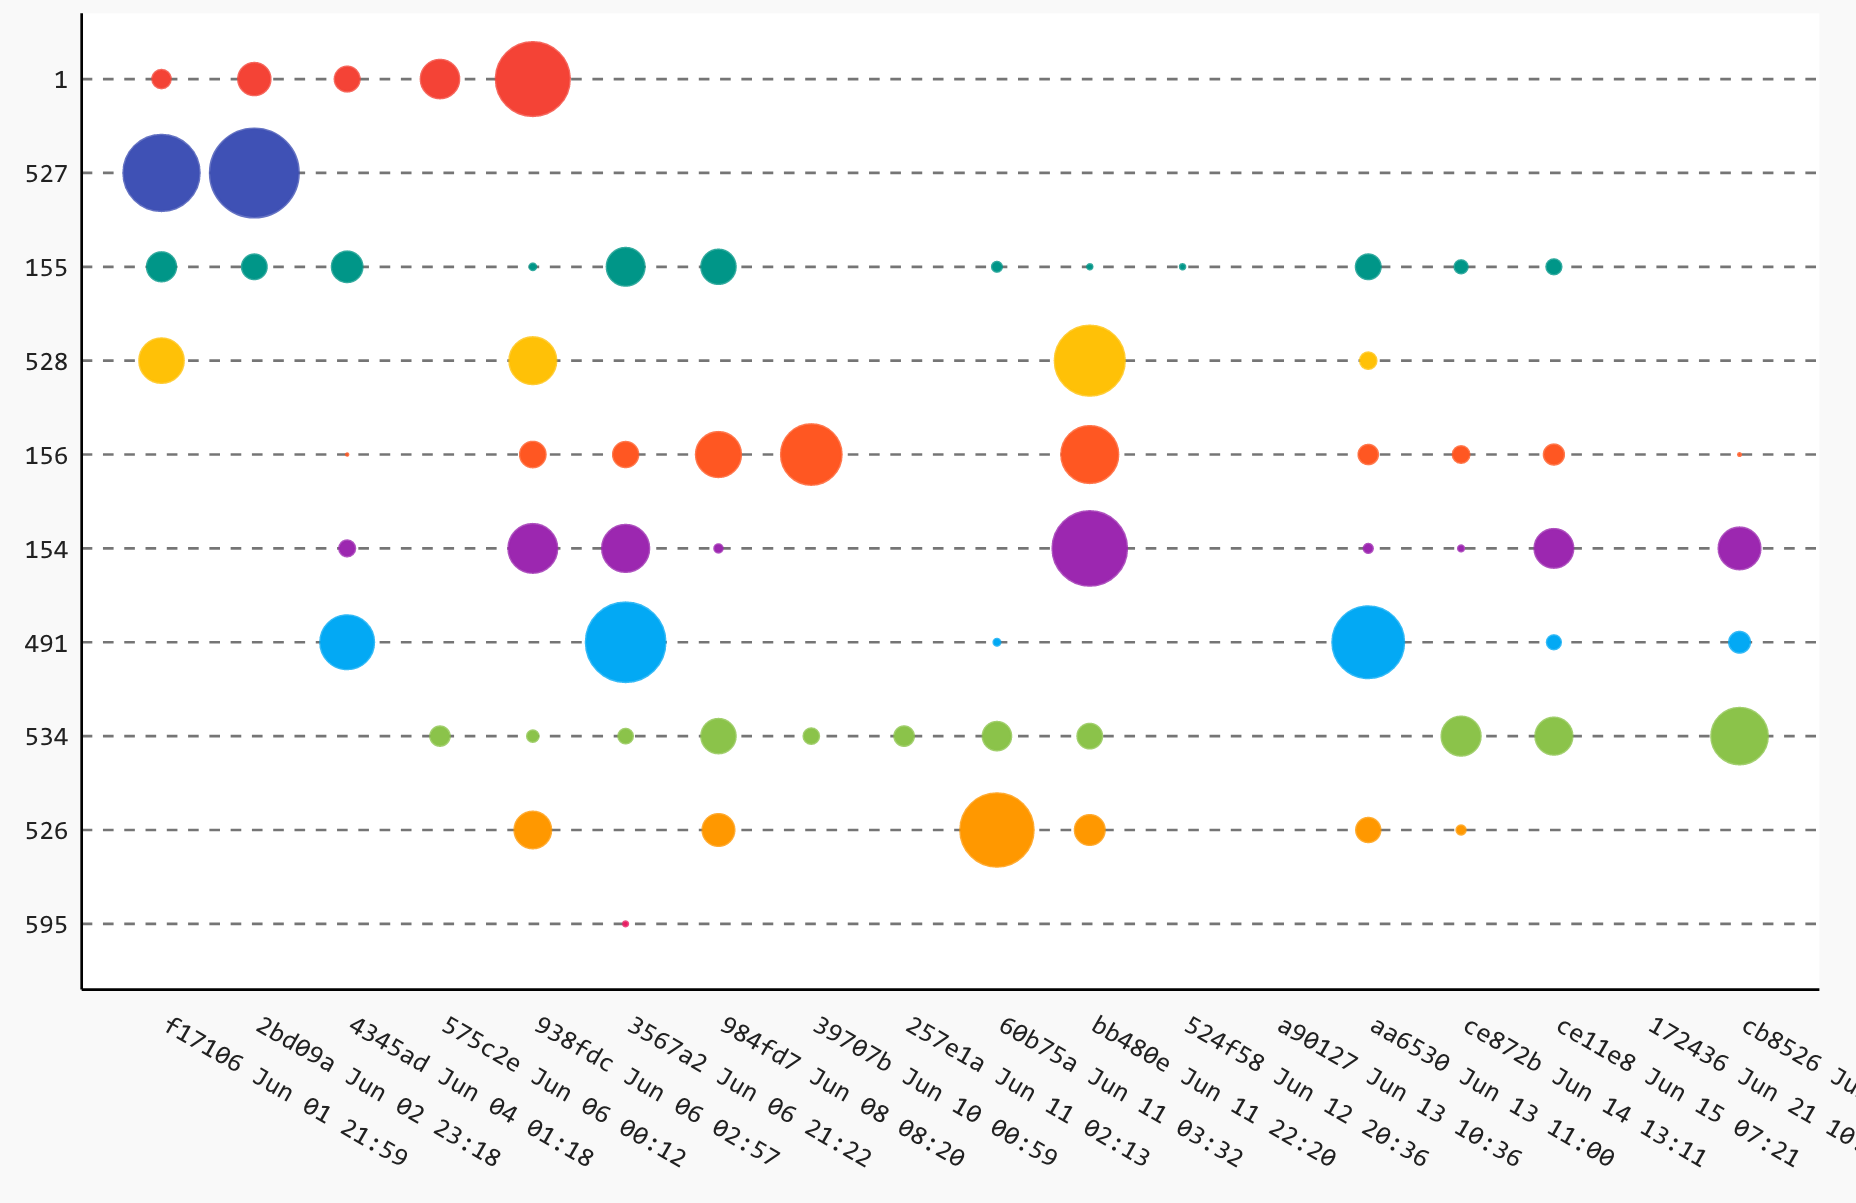
\includegraphics[width=\linewidth]{time_per_user_per_version}
    \caption{Caption here}
    \label{fig:figure1}
  \end{figure}



\section{Tool Availability}

The code of \tool is available online at ...

The images in this paper are screenshots of the actual deployment of the tool which can be found at {https://zeeguu.unibe.ch/api/dashboard}. For the readers of this paper to be able to see the tool in action, they can login with the username and password: guest, dashboardguest!. 
\mltp{we should add a guest/guest username password which is allowed to only visualize things, but not modify anything, and not export anything!}

\section{Conclusion}
The conclusion goes here.




% conference papers do not normally have an appendix


% use section* for acknowledgment
\section*{Acknowledgment}


The authors would like to thank...





% trigger a \newpage just before the given reference
% number - used to balance the columns on the last page
% adjust value as needed - may need to be readjusted if
% the document is modified later
%\IEEEtriggeratref{8}
% The "triggered" command can be changed if desired:
%\IEEEtriggercmd{\enlargethispage{-5in}}

% references section

% can use a bibliography generated by BibTeX as a .bbl file
% BibTeX documentation can be easily obtained at:
% http://mirror.ctan.org/biblio/bibtex/contrib/doc/
% The IEEEtran BibTeX style support page is at:
% http://www.michaelshell.org/tex/ieeetran/bibtex/
%\bibliographystyle{IEEEtran}
% argument is your BibTeX string definitions and bibliography database(s)
%\bibliography{IEEEabrv,../bib/paper}
%
% <OR> manually copy in the resultant .bbl file
% set second argument of \begin to the number of references
% (used to reserve space for the reference number labels box)
\begin{thebibliography}{1}

\bibitem{IEEEhowto:kopka}
H.~Kopka and P.~W. Daly, \emph{A Guide to \LaTeX}, 3rd~ed.\hskip 1em plus
  0.5em minus 0.4em\relax Harlow, England: Addison-Wesley, 1999.

\end{thebibliography}




% that's all folks
\end{document}


